\documentclass[11pt,letterpaper]{article}

\usepackage[letterpaper,top=0.75in,bottom=0.85in,left=0.7in,right=0.7in]{geometry}
\usepackage{graphicx}
\usepackage{xcolor}
\usepackage{listings}
\usepackage{booktabs}
\usepackage{hyperref}
\usepackage{caption}
\usepackage{float}

\hypersetup{
    colorlinks=true,
    linkcolor=blue!60!black,
    urlcolor=blue!60!black,
}

% -----------------------------------------------------------------------------
% VHDL listing style
% -----------------------------------------------------------------------------
\definecolor{codebg}{RGB}{248,248,248}
\definecolor{codekw}{RGB}{0,0,180}
\definecolor{codecmt}{RGB}{0,120,0}
\definecolor{codestr}{RGB}{170,55,20}
\definecolor{codenum}{RGB}{120,120,120}

\lstdefinelanguage{VHDL2008}[]{VHDL}{
    morekeywords={
        library,use,entity,architecture,component,port,map,signal,variable,
        constant,begin,end,process,procedure,function,is,in,out,inout,
        std_logic,std_logic_vector,integer,unsigned,signed,to_integer,
        to_unsigned,to_signed,std,textio,ieee,numeric_std,std_logic_1164,
        rising_edge,falling_edge,wait,until,for,loop,if,then,else,elsif,others,
        severity,note,error,failure,warning,report,after,downto,upto,of,all,
        work,generic
    }
}

\lstset{
    language=VHDL2008,
    basicstyle=\ttfamily\small,
    keywordstyle=\color{codekw}\bfseries,
    commentstyle=\color{codecmt}\itshape,
    stringstyle=\color{codestr},
    numbers=left,
    numberstyle=\tiny\color{codenum},
    stepnumber=1,
    numbersep=6pt,
    backgroundcolor=\color{codebg},
    frame=single,
    rulecolor=\color{black!30},
    tabsize=4,
    showstringspaces=false,
    breaklines=true,
    breakatwhitespace=false,
    breakindent=0pt,
    postbreak=\mbox{\textcolor{red}{$\hookrightarrow$}\space},
    captionpos=b,
    aboveskip=8pt,
    belowskip=8pt,
    xleftmargin=8pt,
    xrightmargin=2pt,
    columns=fullflexible,
    keepspaces=true,
}

\lstdefinestyle{tcl}{
    language=tcl,
    morekeywords={set,puts,if,else,foreach,catch,source,create_ip,set_property,
                  get_ips,get_files,get_filesets,add_files,remove_files,
                  generate_target,export_ip_user_files,update_compile_order,
                  list_property,get_property,format,file,normalize,tail,
                  llength,lsort,info,exists,env,dirname,current_project},
    keywordstyle=\color{codekw}\bfseries,
}

% -----------------------------------------------------------------------------
% Title block
% -----------------------------------------------------------------------------
\title{\textbf{ECEC 661 -- Quiz 1 Submission}\\
       \large RAM-based Shift Register IP}
\author{Gary Pham \texttt{(gp492)}}
\date{\today}

\begin{document}
\maketitle

% =============================================================================
\section{Problem Statement}
% =============================================================================

Simulate the Vivado IP-Catalog \textbf{RAM-based Shift Register}
(\texttt{c\_shift\_ram v12.0}) configured as a 4-bit wide,
6-deep delay line with Clock Enable (CE) and Synchronous Clear (SCLR).

\begin{itemize}
    \item \textbf{Input} \texttt{x} : \texttt{std\_logic\_vector(3 downto 0)}
    \item \textbf{Output} \texttt{z} : \texttt{std\_logic\_vector(3 downto 0)}
    \item \textbf{Control} \texttt{ck}, \texttt{ce}, \texttt{sclr} : \texttt{std\_logic}
    \item \textbf{Behaviour}: \texttt{z} lags \texttt{x} by six rising edges of
        \texttt{ck}; CE freezes the delay line; SCLR clears it synchronously.
\end{itemize}

% =============================================================================
\section{IP Catalog Configuration}
% =============================================================================

The custom IP block \texttt{c\_shift\_ram\_0} is generated from the Vivado
IP Catalog with the parameters listed in Table~\ref{tab:ipconfig}.

\begin{table}[H]
    \centering
    \caption{\texttt{c\_shift\_ram\_0} customisation parameters.}
    \label{tab:ipconfig}
    \begin{tabular}{ll}
        \toprule
        \textbf{Setting} & \textbf{Value} \\
        \midrule
        Shift Register Type       & Fixed Length                      \\
        Width                     & 4                                 \\
        Depth                     & 6                                 \\
        Clock Enable (CE)         & enabled                           \\
        Synchronous Clear (SCLR)  & enabled                           \\
        Async / Sync / Default    & $0$ (hex)                         \\
        Memory Type               & Auto (SRL / distributed / BRAM)   \\
        VLNV                      & \texttt{xilinx.com:ip:c\_shift\_ram:12.0} \\
        \bottomrule
    \end{tabular}
\end{table}

The equivalent Tcl automation from \texttt{scripts/setup.tcl} is:

\begin{lstlisting}[style=tcl,caption={Key IP generation excerpt from setup.tcl}]
create_ip -name c_shift_ram -vendor xilinx.com -library ip -version 12.0 \
          -module_name c_shift_ram_0

set_property -dict [list                        \
    CONFIG.ShiftRegType      {Fixed_Length}     \
    CONFIG.Width             {4}                \
    CONFIG.Depth             {6}                \
    CONFIG.CE                {true}             \
    CONFIG.SCLR              {true}             \
    CONFIG.AsyncInitVal_Hex  {0}                \
    CONFIG.SyncInitVal_Hex   {0}                \
    CONFIG.DefaultData_Hex   {0}                \
] [get_ips c_shift_ram_0]

generate_target {synthesis simulation} [get_ips c_shift_ram_0]
\end{lstlisting}

% =============================================================================
\section{HDL Code}
% =============================================================================

\texttt{user\_logic.vhd} is a thin wrapper that instantiates the IP and
exposes the quiz-required port names (\texttt{x}, \texttt{ck}, \texttt{ce},
\texttt{sclr}, \texttt{z}).

\begin{lstlisting}[caption={user\_logic.vhd},label={lst:userlogic}]
library IEEE;
use IEEE.STD_LOGIC_1164.ALL;
library UNISIM;
use UNISIM.VComponents.all;

-- 4-bit wide, 6-deep RAM-based shift register.  z is x delayed by six
-- rising edges of ck, gated by CE, and cleared synchronously by SCLR.
entity user_logic is
    port (
        x            : in  std_logic_vector(3 downto 0);
        ck, ce, sclr : in  std_logic;
        z            : out std_logic_vector(3 downto 0)
    );
end user_logic;

architecture rtl of user_logic is

    component c_shift_ram_0
        port (
            D    : in  std_logic_vector(3 downto 0);
            CLK  : in  std_logic;
            CE   : in  std_logic;
            SCLR : in  std_logic;
            Q    : out std_logic_vector(3 downto 0)
        );
    end component;

begin

    U_SR : c_shift_ram_0
        port map (
            D    => x,
            CLK  => ck,
            CE   => ce,
            SCLR => sclr,
            Q    => z
        );

end architecture rtl;
\end{lstlisting}

% =============================================================================
\section{Self-Checking Testbench}
% =============================================================================

\texttt{tb\_user\_logic.vhd} drives the DUT through \textbf{11 self-checks}
grouped into five stages:

\begin{enumerate}
    \item \textbf{Initial clear} -- \texttt{z = 0} after SCLR is released.
    \item \textbf{Six-cycle latency} -- driving \texttt{x = 1, 2, \dots, 6}
          produces \texttt{z = 1, 2, \dots, 6} exactly six rising edges later.
    \item \textbf{CE = 0 hold} -- while \texttt{ce} is low, \texttt{z} is
          frozen regardless of \texttt{x}.
    \item \textbf{CE restored} -- data applied while CE was low still needs
          six CE-high edges to emerge on \texttt{z}.
    \item \textbf{Mid-stream SCLR} -- a single SCLR edge wipes the entire
          delay line, forcing \texttt{z = 0}.
\end{enumerate}

\begin{lstlisting}[caption={tb\_user\_logic.vhd -- self-checking testbench},
                   label={lst:tb}]
library ieee;
use ieee.std_logic_1164.all;
use ieee.numeric_std.all;

library std;
use std.textio.all;

entity tb_user_logic is
end entity tb_user_logic;

architecture sim of tb_user_logic is

    constant CK_PERIOD : time := 10 ns;

    signal ck   : std_logic := '0';
    signal ce   : std_logic := '0';
    signal sclr : std_logic := '0';
    signal x    : std_logic_vector(3 downto 0) := (others => '0');
    signal z    : std_logic_vector(3 downto 0);

    signal errors : integer := 0;
    signal checks : integer := 0;

    procedure check_z (
        signal   zsig     : in    std_logic_vector(3 downto 0);
        constant expected : in    integer;
        constant tag      : in    string;
        signal   err_cnt  : inout integer;
        signal   chk_cnt  : inout integer
    ) is
        variable got : integer;
    begin
        got     := to_integer(unsigned(zsig));
        chk_cnt <= chk_cnt + 1;
        if got = expected then
            report "[PASS] " & tag &
                   "  z=" & integer'image(got) severity note;
        else
            report "[FAIL] " & tag &
                   "  got z=" & integer'image(got) &
                   "  expected=" & integer'image(expected) severity error;
            err_cnt <= err_cnt + 1;
        end if;
    end procedure check_z;

begin

    p_ck : process
    begin
        ck <= '0'; wait for CK_PERIOD / 2;
        ck <= '1'; wait for CK_PERIOD / 2;
    end process p_ck;

    dut : entity work.user_logic
        port map (
            x    => x,
            ck   => ck,
            ce   => ce,
            sclr => sclr,
            z    => z
        );

    p_stim : process
    begin
        -- 1. Initial clear
        ce   <= '1';
        sclr <= '1';
        x    <= (others => '0');
        wait until rising_edge(ck);
        wait until rising_edge(ck);
        sclr <= '0';
        wait for 1 ns;
        check_z(z, 0, "post-SCLR init z=0", errors, checks);

        -- 2. Six-cycle latency
        for i in 1 to 6 loop
            x <= std_logic_vector(to_unsigned(i, 4));
            wait until rising_edge(ck);
        end loop;
        wait for 1 ns;
        check_z(z, 1, "latency step 1 (z=x[-6]=1)", errors, checks);

        x <= std_logic_vector(to_unsigned(7, 4));
        wait until rising_edge(ck); wait for 1 ns;
        check_z(z, 2, "latency step 2 (z=x[-6]=2)", errors, checks);

        x <= std_logic_vector(to_unsigned(8, 4));
        wait until rising_edge(ck); wait for 1 ns;
        check_z(z, 3, "latency step 3 (z=x[-6]=3)", errors, checks);

        x <= (others => '0');
        wait until rising_edge(ck); wait for 1 ns;
        check_z(z, 4, "latency step 4 (z=x[-6]=4)", errors, checks);
        wait until rising_edge(ck); wait for 1 ns;
        check_z(z, 5, "latency step 5 (z=x[-6]=5)", errors, checks);
        wait until rising_edge(ck); wait for 1 ns;
        check_z(z, 6, "latency step 6 (z=x[-6]=6)", errors, checks);

        -- 3. CE = 0 holds output
        ce <= '0';
        x  <= std_logic_vector(to_unsigned(9, 4));
        for i in 1 to 3 loop
            wait until rising_edge(ck);
        end loop;
        wait for 1 ns;
        check_z(z, 6, "CE=0 holds z=6 for 3 edges", errors, checks);

        -- 4. CE restored
        ce <= '1';
        for i in 1 to 5 loop
            wait until rising_edge(ck);
        end loop;
        x <= (others => '0');
        wait until rising_edge(ck);
        wait for 1 ns;
        check_z(z, 9, "CE restored, 9 reaches z after 6 edges",
                errors, checks);

        -- 5. Mid-stream SCLR
        for i in 1 to 6 loop
            x <= std_logic_vector(to_unsigned(15, 4));
            wait until rising_edge(ck);
        end loop;
        wait for 1 ns;
        check_z(z, 15, "pre-SCLR: pipeline full of 0xF",
                errors, checks);

        sclr <= '1';
        x    <= (others => '0');
        wait until rising_edge(ck);
        wait for 1 ns;
        check_z(z, 0, "SCLR clears z to 0 in one edge",
                errors, checks);
        sclr <= '0';

        -- Final summary banner
        wait for 5 * CK_PERIOD;
        report LF &
               "+--------------------------------------------------+" & LF &
               "|          tb_user_logic - test summary            |" & LF &
               "+--------------------------------------------------+" & LF &
               "   checks executed : " & integer'image(checks)         & LF &
               "   errors          : " & integer'image(errors)         & LF &
               "+--------------------------------------------------+"
            severity note;

        if errors = 0 then
            report LF &
                   "##       TESTBENCH PASSED - all cases ok        ##"
                severity note;
        else
            report LF &
                   "##  TESTBENCH FAILED - " & integer'image(errors) &
                       " error(s) detected   ##"
                severity failure;
        end if;

        wait;
    end process p_stim;

end architecture sim;
\end{lstlisting}

% =============================================================================
\section{Simulation Results}
% =============================================================================

\subsection{Waveform}

Figure~\ref{fig:wave} shows the xsim behavioural simulation. The clock
\texttt{ck}, enable \texttt{ce}, clear \texttt{sclr}, input \texttt{x}
(unsigned decimal), and output \texttt{z} (unsigned decimal) are shown
along with the running \texttt{checks} counter.

\begin{figure}[H]
    \centering
    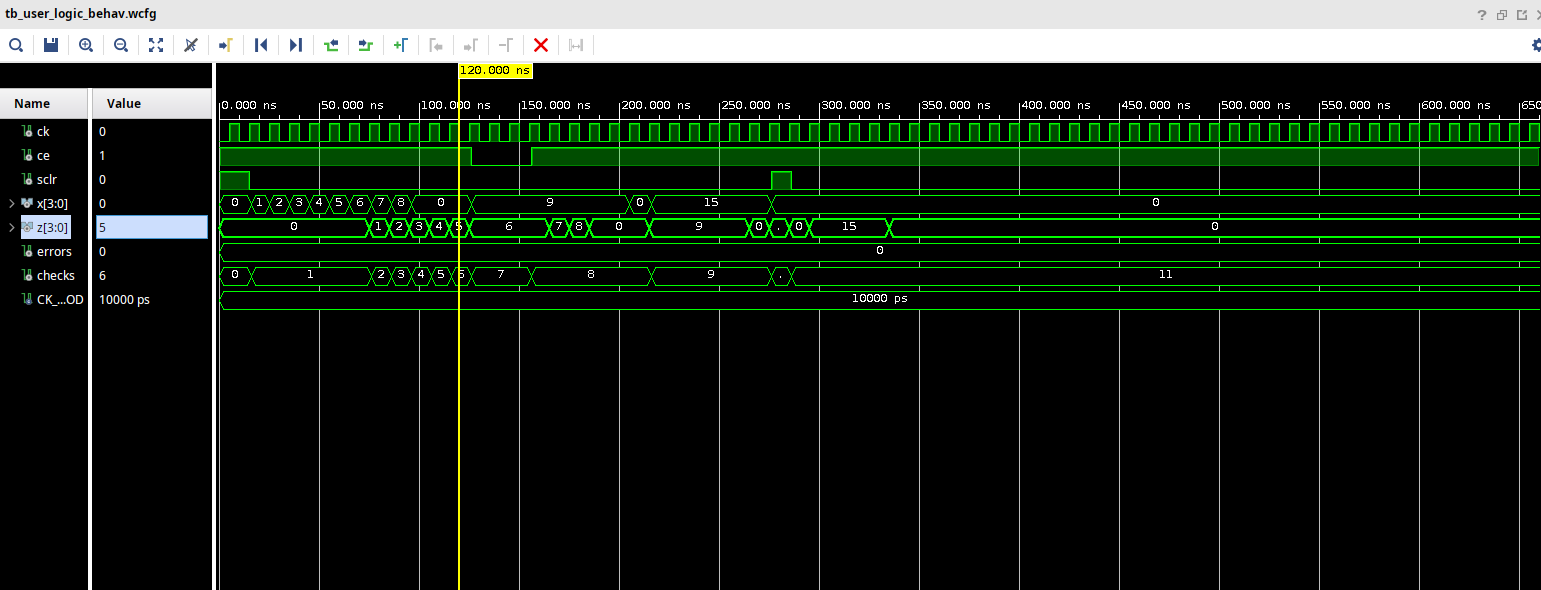
\includegraphics[width=\textwidth]{wave_sim.png}
    \caption{Behavioural simulation of \texttt{tb\_user\_logic}.
             The input \texttt{x} is driven with the sequence
             $1,2,3,4,5,6,7,8,0,0,0$, then $9$ while CE is low, then $15$,
             then $0$ after SCLR.  The output \texttt{z} reproduces the
             same stream exactly six rising edges later
             ($1,2,3,\ldots,6$), holds at $6$ while \texttt{ce} is low,
             then emits $9$ six CE-high edges after enable is restored,
             streams $15$ after the \texttt{0xF} fill, and snaps to $0$
             the instant \texttt{sclr} is pulsed.}
    \label{fig:wave}
\end{figure}

\subsection{Console output}

All 11 self-checks pass:

\begin{lstlisting}[language={},basicstyle=\ttfamily\small,
                    numbers=none,backgroundcolor=\color{codebg},
                    frame=single,breaklines=true,
                    xleftmargin=8pt,xrightmargin=2pt]
[PASS] post-SCLR init z=0
[PASS] latency step 1 (z=x[-6]=1)  z=1
[PASS] latency step 2 (z=x[-6]=2)  z=2
[PASS] latency step 3 (z=x[-6]=3)  z=3
[PASS] latency step 4 (z=x[-6]=4)  z=4
[PASS] latency step 5 (z=x[-6]=5)  z=5
[PASS] latency step 6 (z=x[-6]=6)  z=6
[PASS] CE=0 holds z=6 for 3 edges  z=6
[PASS] CE restored, 9 reaches z after 6 edges  z=9
[PASS] pre-SCLR: pipeline full of 0xF  z=15
[PASS] SCLR clears z to 0 in one edge  z=0

+--------------------------------------------------+
|          tb_user_logic - test summary            |
+--------------------------------------------------+
   checks executed : 11
   errors          : 0
+--------------------------------------------------+

##       TESTBENCH PASSED - all cases ok        ##
\end{lstlisting}

% =============================================================================
\section{Conclusion}
% =============================================================================

The RAM-based Shift Register IP operates exactly as specified:
output \texttt{z} lags input \texttt{x} by six rising edges of \texttt{ck},
Clock Enable freezes the delay line without corrupting its contents, and
a single edge with \texttt{sclr = 1} clears every stage synchronously.
All eleven self-checks in the testbench return \texttt{[PASS]} and the
simulator terminates with the \textit{TESTBENCH PASSED} banner.

\end{document}
